\documentclass[a4paper,10pt]{article}
\usepackage[utf8]{inputenc}
\usepackage{amstext}
\usepackage{listings}
\usepackage{graphicx}
\usepackage{subfigure}
\usepackage[T1]{fontenc}
\usepackage[utf8]{inputenc}
\usepackage[font=small,labelfont=bf]{caption}
\usepackage{float}
\usepackage[dutch]{babel}
\usepackage[section]{placeins}

\DeclareCaptionLabelFormat{andtable}{#1~#2  \&  \tablename~\thetable}


%opening
\title{Betrouwbare end-to-end communicatie}
\author{Patrick van Looy \& Bram Leenders}

\begin{document}

\maketitle

\section{Inleiding}
Bij het opzetten van sensornetwerken, kan het zijn dat twee nodes niet in elkaars zendbereik vallen. In een dergelijk geval kan een tussenliggende node helpen door berichten door te sturen. Zo kunnen nodes als schakels in een ketting gebruikt worden om een groter bereik mogelijk te maken.

Een dergelijke constructie is een stuk gecompliceerder dan directe communicatie tussen twee nodes, omdat voor betrouwbare communicatie het zenden van ontvangstbevestigingen nodig is. Het communiceren binnen een groep nodes is daarom ook geen onderdeel van de standaard meegeleverde libraries. Het doel van dit onderzoek was het mogelijk maken van communicatie via nodes, gebruikmakend van de functionaliteit die wel door Arduino's geleverd wordt.

\section{Probleemstelling}
Om het probleem overzichtelijk te houden, is het aantal nodes in deze proef beperkt tot drie. Er is een zender, een ontvanger en een doorsturende node. Omdat het aantal nodes beperkt is, is er maar \'e\'en mogelijk pad. Hierdoor kan het pad vooraf vastgelegd worden, dit heet ook wel statische routering.

De uiteindelijke opstelling moet de zender de garantie geven dat een bericht uiteindelijk ontvangen wordt door de ontvanger via de tussenliggende node.

We willen nu weten of het mogelijk is om via een multihopnetwerk betrouwbare end-to-end communicatie te garanderen. 
Specifiek verwoord: dit onderzoek heeft als doel om een protocol te ontwikkelen dat de juiste packetvolgorde en de volledigheid (er ontbreken geen packets) garandeert. Van dit protocol wordt tevens een implementatie gegeven.

\section{Protocol}
Zoals gezegd is dient het protocol te garanderen dat er geen packets wegvallen tijdens het verzenden en packets de juiste volgorde te behouden. Om dit te garanderen, kan gebruik worden gemaakt van het alternating bit protocol (ABP). Dit protocol stuurt een nummer -een bit- mee met een pakket, wanneer de ontvanger het ontvangt stuurt deze bevestiging met datzelfde nummer terug. Indien de zender een bevestiging met het correcte (laatst verzonden) nummer ontvangt, hoogt deze een counter met een op en stuurt deze het volgende pakket.

Figuur~\ref{fig:flow} illustreert het pad dat een pakket met bijbehorende bevestiging aflegt. Figuur~\ref{fig:roles} toont de verschillende staten waarin een zender/herhaler/ontvanger zich kan bevinden en de transities tussen deze staten.

\begin{figure}[ht!]
    \centering
    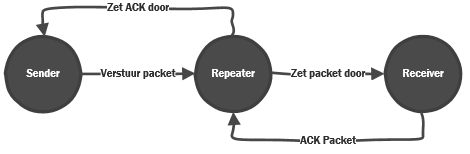
\includegraphics[width=0.8\textwidth]{flow.png}
    \caption{}
    \label{fig:flow}
\end{figure}

\begin{figure}[ht!]
    \begin{minipage}{\textwidth}
        \begin{minipage}{0.49\textwidth}
            \centering
            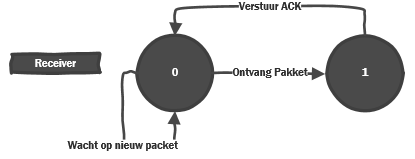
\includegraphics[width=\textwidth]{receiver.png}
            \caption*{Ontvanger Arduino}
        \end{minipage}
        \hfill
        \begin{minipage}{0.49\textwidth}
            \centering
            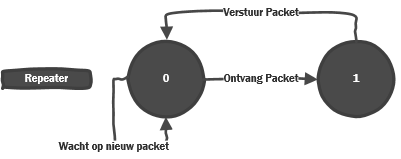
\includegraphics[width=\textwidth]{repeater.png}
            \caption*{Herhaler Arduino}
        \end{minipage}
        \hfill\centering
        \begin{minipage}{0.8\textwidth}
            \centering
            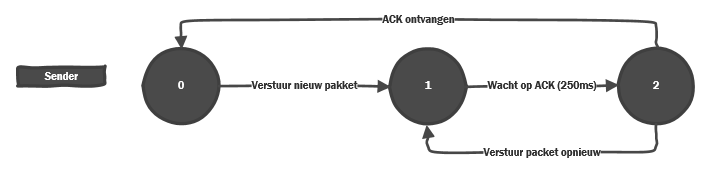
\includegraphics[width=0.95\textwidth]{sender.png}
            \caption*{Zender Arduino}
        \end{minipage}
    \caption{State-diagram Alternating Bit Protocol voor de drie communicerende Arduino's.}
    \label{fig:roles}
    \end{minipage}
\end{figure}

\section{Implementatie}
Onze implementatie gebruikt niet een enkele bit als identificatie van een pakket, maar een getal. Conceptueel verandert dit niets aan het protocol, maar het biedt wel de mogelijkheid voor later uitbreiding. Zo geldt niet langer de restrictie dat er slechts \'e\'en oud pakket in het netwerk mag zitten. Onze implementatie werkt dus ook als oudere berichten (e.g. tien berichten terug) nog ronddolen in het netwerk.

Tevens stuurt de ontvanger een ACK terug die niet de identificatiecode bevat, maar de negatieve waarde hiervan. Hierdoor is het direct duidelijk of een pakket een bevestiging is (indien de code kleiner dan 0 is), of echte data bevat. Dit helpt om ook in grote netwerken ervoor te zorgen dat een zender niet zijn zelf verzonden bericht als ACK kan lezen.

Verder moet de communcatie op zowel korte als lange afstand betrouwbaar zijn, ook dit moet getest worden.

\section{Test methodologie en resultaten}
De implementatie, waarvan de code is bijgevoegd in appendix~\ref{sec:code}, is in verschillende vormen getest:
\begin{itemize}
	\item De zender, herhaler en ontvanger allemaal binnen elkaars ontvangstbereik.
	\item De zender en herhaler respectievelijk de herhaler en ontvanger binnen ontvangstbereik, maar zender en ontvanger buiten ontvangstbereik.
	\item Alleen zender en ontvanger binnen ontvangstbereik; herhaler buiten bereik.
\end{itemize}
Omdat er gebruik gemaakt is van statistische routering, is het geen optie voor de zender en ontvanger om direct te communiceren. In de eerste twee gevallen verloopt de communicatie via de herhaler; in het derde geval kan geen verbinding worden opgezet omdat de herhaler niet bereikbaar is.

\begin{figure}[ht!]
    \begin{minipage}{\textwidth}
        \begin{minipage}{0.3\textwidth}
            \centering
            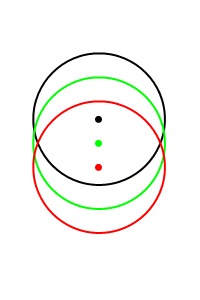
\includegraphics[width=0.9\textwidth]{een.jpg}
            \caption*{Alles direct bereikbaar}
        \end{minipage}
        \hfill
        \begin{minipage}{0.3\textwidth}
            \centering
            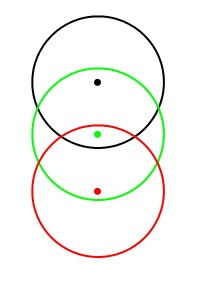
\includegraphics[width=0.9\textwidth]{twee.jpg}
            \caption*{Ontvanger bereikbaar via herhaler}
        \end{minipage}
        \hfill
        \begin{minipage}{0.3\textwidth}
            \centering
            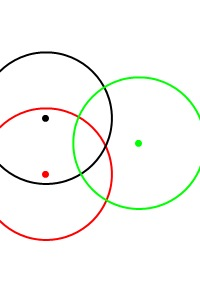
\includegraphics[width=0.9\textwidth]{drie.jpg}
            \caption*{Herhaler onbereikbaar}
        \end{minipage}
	\caption{Drie mogelijke scenario's; zwart is de verzender, groen is de herhaler en rood is de ontvanger.}
    \end{minipage}
\end{figure}

Op zowel korte als lange afstand (tussen zender en ontvanger zo'n veertig meter, overbrugd via herhalers) bleken de nodes in staat te zijn alle packets succesvol af te leveren. Eventueel packet loss wordt door het algoritme gedetecteerd, en de ontbrekende packets worden opnieuw gestuurd totdat deze ontvangen zijn. In deze gevallen werkt het protocol dus zoals gewensd, in het derde geval werkt het protocol niet maar werd dit ook niet verwacht. Immers, dit scenario valt buiten de oorspronkelijke eisen.

\section{Conclusie}
Concluderend, het is wel degelijk mogelijk om via een multihopnetwerk betrouwbare end-to-end communicatie te garanderen. Bij het uitgevoerde onderzoek zijn de resultaten verassend goed. Over een grote afstand waarbij veel mogelijke obstakels en stoorzenders aanwezig waren, bleken de nodes in staat te zijn nagenoeg alle individuele packets succesvol af te leveren bij de desbetreffende ontvanger.

In gedachten nemend dat een (sensor)netwerk op een veel grotere schaal nog steeds betrouwbaar moet zijn, is het wel verstandig ervoor te zorgen dat er altijd twee andere nodes bereikt kunnen worden. Op deze manier is het veiliger om te zeggen dat een packet altijd bij zijn bestemming aankomt, omdat je er dan rekening mee houdt dat er eventueel een node kapot zou kunnen gaan of uitvalt. Mocht dit gebeuren, dan kan de andere node die binnen bereik is de taak van de kapotte node overnemen. Dit valt echter buiten de scope van dit onderzoek, en kan in een volgend onderzoek verder uitgewerkt worden.

Verder onderzoek zou gedaan kunnen worden naar het dynamisch maken van het netwerk. Op die manier is het veel gemakkelijker om nodes te verwijderen of toe te voegen in een netwerk en gaat het netwerk dus ook beter om met een node die kapot gaat of uitvalt. Om deze functionaliteit te kunnen bieden moet het protocol nog veel aangepast worden en is het nodig om dynamische routering te implementeren.

\newpage
\appendix
\section{Bijlage 1 - Code}
\label{sec:code}
% xxxxxxxxxxxxxxxxxxxxxxxxx Code Snippet STARTS xxxxxxxxxxxxxxxxxxxxxx
\lstset{
  language=C,                     % choose the language of the code
  stepnumber=1,                   % the step between two line-numbers. If it's 1, each line will be numbered
  basicstyle=\footnotesize,
 % numbersep=5pt,                 % how far the line-numbers are from the code
%  backgroundcolor=\color{white}, % choose the background color. You must add \usepackage{color}
  showspaces=false,               % show spaces adding particular underscores
  showstringspaces=false,         % underline spaces within strings
  showtabs=false,                 % show tabs within strings adding particular underscores
  tabsize=4,                      % sets default tabsize to 2 spaces
  captionpos=t,                   % sets the caption-position to top
  breaklines=true,                % sets automatic line breaking
  breakatwhitespace=true,         % sets if automatic breaks should only happen at whitespace
 % title=\lstname,                % show the filename of files included with \lstinputlisting;
 % identifierstyle=\color{identifierColor},
 % caption={Array of Pointers to Strings},
 % frame=lrtb,
 % keywordstyle=\color{purple},         % keyword style
 % commentstyle=\color{blue},           % comment style
 % stringstyle=\color{violet},          % string literal style
 belowcaptionskip = 0.2in,            % Space below caption
 abovecaptionskip = 0.2in             % Space above caption
}
% \lstset{language=C}
\begin{lstlisting}
/*
    Positioning system for Arduino One with RF24 radio chip
*/
#include <SPI.h>
#include "nRF24L01.h"
#include "RF24.h"
#include "printf.h"
#include "MatrixMath.h"

#define N (3)
// Kunstmatige waarde voor Z coordinaten
#define Z 1.0
// Percentage verschil (0 < MAX_DIFF <= 1) dat tussen twee metingen mag zitten.
#define MAX_DIFF (0.25)
// Percentage dat de nieuwste meting in het gemiddelde meetelt (0 < WEIGHT <= 1)
// Bij WEIGHT=1 wordt er geen gemiddelde bijgehouden, maar is de nieuwste meting de enige die meetelt.
#define WEIGHT (0.2)

RF24 radio(3, 9);
unsigned long radiotime;
unsigned long audiotime;
unsigned long timelimit = 50000LL;
uint8_t activeBeacon;

float pos[4][2] = { // Positions van de beacons; pos[1][1] is de y positie van beacon 1
    {0.0, 75.0},
    {72.0, 0.0},
    {294.0, 0.0},
    {372.0, 136.0}
};

float D[4];


void setup() {
  // initialize the serial communication:
  Serial.begin(9600);
  printf_begin();

  // Setup and configure rf radio
  radio.begin();
  radio.setRetries(0,0);

  radio.setDataRate(RF24_2MBPS);
  radio.setChannel(76);
  radio.setPayloadSize(1);
  radio.openReadingPipe(1, 0xdeadbeefa1LL);
  radio.openWritingPipe(0xdeadbeefa1LL);
  radio.startListening();
  radio.setAutoAck(false);
}

void loop() {
  while(radio.available()) { 
    radio.read(&activeBeacon, sizeof(uint8_t)); 
  }
  while (! radio.available());

  radiotime = micros();
  radio.read( &activeBeacon, sizeof(uint8_t));

  if(activeBeacon > 3) { return; }

  while(analogRead(A0) < 50) {
    audiotime = micros();
    if(audiotime - radiotime > timelimit) {
      return; 
    }
  }
  
  float diff = audiotime - radiotime;
  diff = diff * 0.03432; // Afstand tot beacon in cm

  //Zwak uitschieters een beetje af: max 30% increase
  if(diff > (D[activeBeacon]* (1.0 + MAX_DIFF)) && D[activeBeacon] > 0) {
    diff = D[activeBeacon] * (1.0 + MAX_DIFF);
  }
  
  if(diff < (D[activeBeacon]* (1.0 - MAX_DIFF))) {
    diff = D[activeBeacon]*(1.0 - MAX_DIFF);
  }
  
  D[activeBeacon] = D[activeBeacon]*(1.0 - WEIGHT) + diff*WEIGHT; // Weer schuivend gemiddelde */
  //D[activeBeacon] = diff;

  if(activeBeacon == 3) {
    calcPosition();
  }
}

float A[N][N];
float B[N];

void calcPosition() {
    // Relatieve afstanden tussen de nodes; gebruikt node 3 nog niet!
    A[0][0] = 2*pos[1][0] - 2*pos[0][0]; A[0][1] = 2*pos[1][1] - 2*pos[0][1]; A[0][2] = Z;
    A[1][0] = 2*pos[2][0] - 2*pos[1][0]; A[1][1] = 2*pos[2][1] - 2*pos[1][1]; A[1][2] = Z;
    A[2][0] = 2*pos[0][0] - 2*pos[2][0]; A[2][1] = 2*pos[0][1] - 2*pos[2][1]; A[2][2] = Z;
    Matrix.Invert((float*)A,N);

    B[0] = (D[0]*D[0]) - (D[1]*D[1]) - (pos[0][0]*pos[0][0]) + (pos[1][0]*pos[1][0]) - (pos[0][1]*pos[0][1]) + (pos[1][1]*pos[1][1]);
    B[1] = (D[1]*D[1]) - (D[2]*D[2]) - (pos[1][0]*pos[1][0]) + (pos[2][0]*pos[2][0]) - (pos[1][1]*pos[1][1]) + (pos[2][1]*pos[2][1]);
    B[2] = (D[2]*D[2]) - (D[0]*D[0]) - (pos[2][0]*pos[2][0]) + (pos[0][0]*pos[0][0]) - (pos[2][1]*pos[2][1]) + (pos[0][1]*pos[0][1]);
    
    float P3[N];
    Matrix.Multiply((float*)A,(float*)B,N,N,1,(float*)P3);
    printf("Position (P3): (%d,%d)\n", (int) P3[0], (int) P3[1]);
    

    // Relatieve afstanden tussen de nodes; gebruikt node 2 nog niet!
    A[0][0] = 2*pos[1][0] - 2*pos[0][0]; A[0][1] = 2*pos[1][1] - 2*pos[0][1]; A[0][2] = Z;
    A[1][0] = 2*pos[3][0] - 2*pos[1][0]; A[1][1] = 2*pos[3][1] - 2*pos[1][1]; A[1][2] = Z;
    A[2][0] = 2*pos[0][0] - 2*pos[3][0]; A[2][1] = 2*pos[0][1] - 2*pos[3][1]; A[2][2] = Z;
    Matrix.Invert((float*)A,N);

    B[0] = (D[0]*D[0]) - (D[1]*D[1]) - (pos[0][0]*pos[0][0]) + (pos[1][0]*pos[1][0]) - (pos[0][1]*pos[0][1]) + (pos[1][1]*pos[1][1]);
    B[1] = (D[1]*D[1]) - (D[3]*D[3]) - (pos[1][0]*pos[1][0]) + (pos[3][0]*pos[3][0]) - (pos[1][1]*pos[1][1]) + (pos[3][1]*pos[3][1]);
    B[2] = (D[3]*D[3]) - (D[0]*D[0]) - (pos[3][0]*pos[3][0]) + (pos[0][0]*pos[0][0]) - (pos[3][1]*pos[3][1]) + (pos[0][1]*pos[0][1]);
    float P2[N];
    Matrix.Multiply((float*)A,(float*)B,N,N,1,(float*)P2);
    printf("Position (P2): (%d,%d)\n", (int) P2[0], (int) P2[1]);
    
    
    // Relatieve afstanden tussen de nodes; gebruikt node 1 nog niet!
    A[0][0] = 2*pos[2][0] - 2*pos[0][0]; A[0][1] = 2*pos[2][1] - 2*pos[0][1]; A[0][2] = Z;
    A[1][0] = 2*pos[3][0] - 2*pos[2][0]; A[1][1] = 2*pos[3][1] - 2*pos[2][1]; A[1][2] = Z;
    A[2][0] = 2*pos[0][0] - 2*pos[3][0]; A[2][1] = 2*pos[0][1] - 2*pos[3][1]; A[2][2] = Z;
    Matrix.Invert((float*)A,N);
   
    B[0] = (D[0]*D[0]) - (D[2]*D[2]) - (pos[0][0]*pos[0][0]) + (pos[2][0]*pos[2][0]) - (pos[0][1]*pos[0][1]) + (pos[2][1]*pos[2][1]);
    B[1] = (D[2]*D[2]) - (D[3]*D[3]) - (pos[2][0]*pos[2][0]) + (pos[3][0]*pos[3][0]) - (pos[2][1]*pos[2][1]) + (pos[3][1]*pos[3][1]);
    B[2] = (D[3]*D[3]) - (D[0]*D[0]) - (pos[3][0]*pos[3][0]) + (pos[0][0]*pos[0][0]) - (pos[3][1]*pos[3][1]) + (pos[0][1]*pos[0][1]);
    float P1[N];
    Matrix.Multiply((float*)A,(float*)B,N,N,1,(float*)P1);
    printf("Position (P1): (%d,%d)\n", (int) P1[0], (int) P1[1]);
    
    
    // Relatieve afstanden tussen de nodes; gebruikt node 0 nog niet!
    A[0][0] = 2*pos[2][0] - 2*pos[1][0]; A[0][1] = 2*pos[2][1] - 2*pos[1][1]; A[0][2] = Z;
    A[1][0] = 2*pos[3][0] - 2*pos[2][0]; A[1][1] = 2*pos[3][1] - 2*pos[2][1]; A[1][2] = Z;
    A[2][0] = 2*pos[1][0] - 2*pos[3][0]; A[2][1] = 2*pos[1][1] - 2*pos[3][1]; A[2][2] = Z;
    Matrix.Invert((float*)A,N);
   
    B[0] = (D[1]*D[1]) - (D[2]*D[2]) - (pos[1][0]*pos[1][0]) + (pos[2][0]*pos[2][0]) - (pos[1][1]*pos[1][1]) + (pos[2][1]*pos[2][1]);
    B[1] = (D[2]*D[2]) - (D[3]*D[3]) - (pos[2][0]*pos[2][0]) + (pos[3][0]*pos[3][0]) - (pos[2][1]*pos[2][1]) + (pos[3][1]*pos[3][1]);
    B[2] = (D[3]*D[3]) - (D[1]*D[1]) - (pos[3][0]*pos[3][0]) + (pos[1][0]*pos[1][0]) - (pos[3][1]*pos[3][1]) + (pos[1][1]*pos[1][1]);
    float P0[N];
    Matrix.Multiply((float*)A,(float*)B,N,N,1,(float*)P0);
    printf("Position (P0): (%d,%d)\n", (int) P0[0], (int) P0[1]);
    
    // Bereken het gemiddelde van de verschillende metingen:
    int avg[N];
    avg[0] = (int) (P0[0] + P1[0] + P2[0] + P3[0]) / 4.0;
    avg[1] = (int) (P0[1] + P1[1] + P2[1] + P3[1]) / 4.0;
    avg[2] = (int) (P0[2] + P1[2] + P2[2] + P3[2]) / 4.0;
  
    printf("Position: (%d,%d)\n\n", avg[0], avg[1]);
}
\end{lstlisting}

\end{document}
